%\section{Theoretical Introduction}
\label{sec:cap3}

This chapter presents the theoretical background necessary to understand the techniques and concepts explored in this dissertation. It introduces the reliability challenges of SRAM-based FPGAs, examines fault-tolerance techniques such as N-Modular Redundancy (NMR) and Dynamic Partial Reconfiguration (DPR), discusses memory scrubbing mechanisms, and outlines the principles of fault injection for resilience evaluation. 

\section{Reliability Challenges in SRAM-based FPGAs}
SRAM-based FPGAs are widely adopted for their flexibility, performance, and reconfigurability. However, their configuration memory (\gls{cram}) and user logic are highly susceptible to soft errors induced by radiation, electromagnetic interference, or aging effects. These transient faults may alter logic functionality or corrupt stored data, potentially leading to malfunction or complete system failure. Understanding the nature, frequency, and impact of these faults is critical for developing effective mitigation strategies.

%%Types of Errors
\usetikzlibrary{shapes.geometric, arrows}

\tikzstyle{block} = [rectangle, rounded corners, minimum width=4cm, minimum height=1cm, text centered, draw=black, fill=blue!20]
\tikzstyle{subblock} = [rectangle, rounded corners, minimum width=3.5cm, minimum height=0.8cm, text centered, draw=black, fill=green!20]
\tikzstyle{arrow} = [thick,->,>=stealth]

\begin{figure}[ht]
\centering
\begin{adjustbox}{max width=\textwidth}
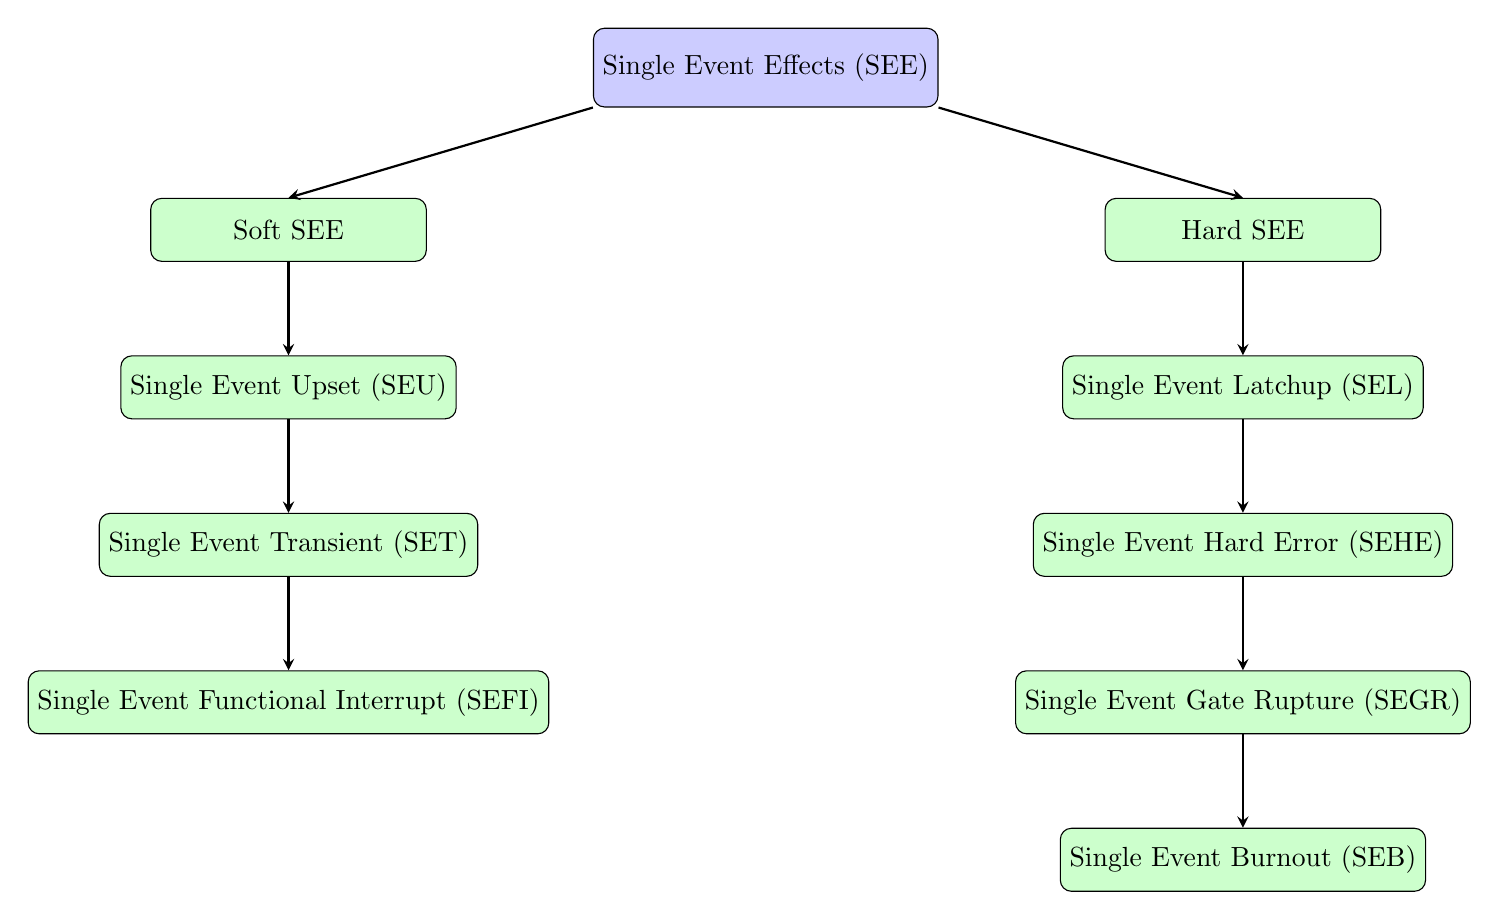
\begin{tikzpicture}[node distance=1.5cm]

% Top-level SEE
\node (see) [block] {Single Event Effects (SEE)};

% Soft SEE
\node (soft) [subblock, below left of=see, xshift=-5cm, yshift=-1cm] {Soft SEE};
\node (seu) [subblock, below of=soft, yshift=-0.5cm] {Single Event Upset (SEU)};
\node (set) [subblock, below of=seu, yshift=-0.5cm] {Single Event Transient (SET)};
\node (sefi_soft) [subblock, below of=set, yshift=-0.5cm] {Single Event Functional Interrupt (SEFI)};

% Hard SEE
\node (hard) [subblock, below right of=see, xshift=5cm, yshift=-1cm] {Hard SEE};
\node (sel) [subblock, below of=hard, yshift=-0.5cm] {Single Event Latchup (SEL)};
\node (sehe) [subblock, below of=sel, yshift=-0.5cm] {Single Event Hard Error (SEHE)};
\node (segr) [subblock, below of=sehe, yshift=-0.5cm] {Single Event Gate Rupture (SEGR)};
\node (seb) [subblock, below of=segr, yshift=-0.5cm] {Single Event Burnout (SEB)};

% Arrows from SEE to Soft and Hard
\draw [arrow] (see.south west) -- (soft.north);
\draw [arrow] (see.south east) -- (hard.north);

% Arrows within Soft SEE
\draw [arrow] (soft.south) -- (seu.north);
\draw [arrow] (seu.south) -- (set.north);
\draw [arrow] (set.south) -- (sefi_soft.north);

% Arrows within Hard SEE
\draw [arrow] (hard.south) -- (sel.north);
\draw [arrow] (sel.south) -- (sehe.north);
\draw [arrow] (sehe.south) -- (segr.north);
\draw [arrow] (segr.south) -- (seb.north);

\end{tikzpicture}
\end{adjustbox}
\caption{Classification of Single Event Effects (SEE) into Soft SEE and Hard SEE with their subtypes.}
\label{fig:see_hard_soft}
\end{figure}

%%%%%%%%%%%%%%%%%%%%%%%%%%%%%%%%%%%%%%%%%%%%%%%%%%%%%%%%%%%%%%%%%%%%%%%%%%%

\section{N-Modular Redundancy (NMR)}
\gls{nmr} is a fault-masking technique where multiple identical modules operate in parallel, and a majority voter determines the correct output. While \gls{tmr} (Triple Modular Redundancy) is the most common case, extending to higher-order NMR provides increased fault tolerance at the expense of resource overhead. This section explains the mathematical basis of NMR, voter design considerations, fault coverage properties, and limitations regarding permanent resource degradation.

\section{Dynamic Partial Reconfiguration (DPR)}
\gls{dpr} enables the selective reprogramming of specific FPGA regions during runtime without disrupting the operation of unaffected modules. By targeting only the faulty portions of the design, DPR reduces downtime and resource waste compared to full device reprogramming. This section describes the internal mechanisms of DPR, design partitioning strategies, and how it complements redundancy to achieve self-repairing FPGA systems.

\section{Memory Scrubbing Techniques}
Configuration memory scrubbing is a proactive approach that periodically reads and corrects the FPGA configuration to prevent error accumulation. This section discusses different scrubbing approaches, including blind scrubbing, readback-and-verify, and adaptive scrubbing. It also analyzes trade-offs between error coverage, bandwidth consumption, and system availability.

\section{Fault Injection Principles}
Fault injection is an essential method for evaluating the robustness of fault-tolerant FPGA designs. By deliberately introducing controlled errors into the system, researchers can analyze failure modes, verify mitigation strategies, and quantify reliability metrics. This section explains fault injection models (bit-flip, stuck-at), implementation techniques (simulation-based, emulation-based, on-chip), and evaluation criteria.

\section{Fault Injection Overview}

\subsection{Fault Injection Models}
This subsection describes the types of faults that can be injected into FPGA systems. Proper modeling is crucial to evaluate system reliability and test mitigation strategies.

\subsubsection{Bit-Flip Faults}
Bit-flip faults simulate transient errors, such as single-event upsets, in memory cells or configuration bits. These faults are temporary and can occur randomly due to radiation or electromagnetic interference. Studying bit-flip faults helps evaluate the effectiveness of runtime error detection and correction mechanisms.

\subsubsection{Stuck-At Faults}
Stuck-at faults represent permanent logical errors where a signal line is stuck at a logical '0' or '1'. These faults can occur due to manufacturing defects or severe electrical stress. Injecting stuck-at faults allows assessment of system behavior under permanent defects and validates repair mechanisms such as partial dynamic reconfiguration.

\subsection{Implementation Techniques}
This subsection presents the main approaches for performing fault injection in FPGA systems. Each technique has advantages and trade-offs regarding accuracy, speed, and realism.

\subsubsection{Simulation-Based Fault Injection}
Simulation-based techniques introduce faults into software models of the system. This method allows early evaluation without physical hardware and can test a large number of scenarios quickly. However, it may not capture all hardware-specific effects.

\subsubsection{Emulation-Based Fault Injection}
Emulation-based fault injection uses a hardware-in-the-loop setup, often leveraging FPGA prototypes or development boards. This method provides a more accurate assessment than simulation and allows testing of real hardware timing and interactions.

\subsubsection{On-Chip Fault Injection}
On-chip fault injection directly manipulates configuration memory, logic cells, or peripheral interfaces in the FPGA. This approach provides the most realistic evaluation of system behavior under actual fault conditions but may require sophisticated instrumentation and careful safety measures.

\subsection{Evaluation Criteria}
Defining proper evaluation criteria is essential to measure the impact of injected faults and assess mitigation strategies.

\subsubsection{Fault Coverage}
Fault coverage quantifies the proportion of injected faults that are successfully detected or mitigated by the system. High coverage indicates a robust design capable of handling the expected fault rate.

\subsubsection{Error Latency}
Error latency measures the time between fault occurrence and detection or correction. Low latency is critical for systems requiring real-time reliability, such as aerospace or automotive applications.

\subsubsection{Recovery Time}
Recovery time indicates how quickly the system can return to normal operation after a fault. Techniques like NMR, DPR, and memory scrubbing aim to minimize recovery time to maintain continuous operation.


\section{Reliability Metrics and Evaluation Methods}
Assessing the effectiveness of fault-tolerance techniques requires quantitative metrics such as Mean Time Between Failures (MTBF), fault coverage, and error latency. This section introduces these metrics, outlines statistical approaches to evaluate system reliability, and highlights how they guide design trade-offs in FPGA-based systems.

